% BEGIN: j2r3k4l5t6y7
\documentclass{report}
\usepackage[total={7in,9in}]{geometry}
\usepackage{graphicx}
\usepackage{amsmath}
\usepackage{amssymb}
\usepackage{tikz}

\begin{document}
\begin{center}
    \Large\textbf{SPM Trial Exam 2022}

    \textbf{Johor}

    \vspace{1cm}
    \normalsize\textbf{Paper 1}

    \vspace{1cm}

    \begin{enumerate}
        \item Diagram 1, shows a sector of a circle with centre $O$.

              \begin{center}
                  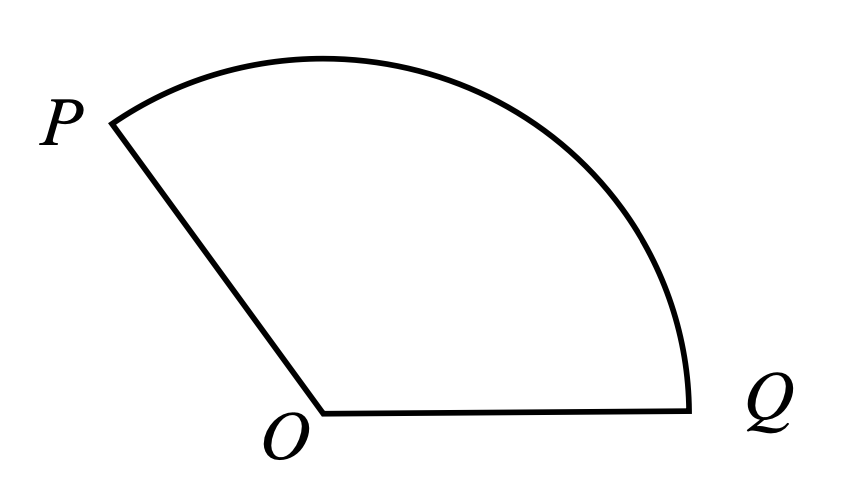
\includegraphics[width=0.3\textwidth]{./assets/d1.png}
              \end{center}

              The sector is formed from a piece of wire of length 95 cm. It is given that the
              length of arc PQ is 55 cm, find $\angle$POQ in radians.\\~\\

              \textbf{Sol.}
              \begin{flalign*}
                  OQ          & = PQ = \dfrac{95-55}{2} = 20                        &              \\
                  20          & \cdot \angle{POQ} = 55                                             \\
                  \angle{POQ} & = \dfrac{55}{20} = \dfrac{11}{4} = 2.75 \text{ rad} & \blacksquare
              \end{flalign*}

              \vfill\null

        \item Diagram 2 shows part of the graph $y$ against $x$.

              \begin{center}
                  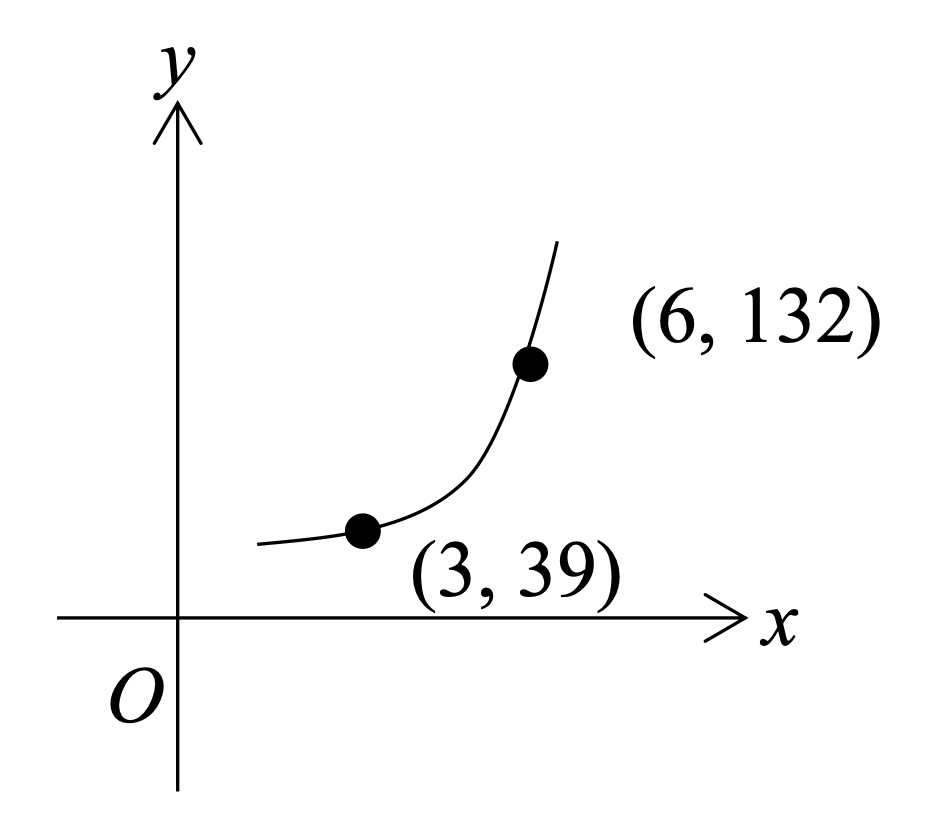
\includegraphics[width=0.3\textwidth]{./assets/d2.png}
              \end{center}

              It is known that the linear equation that related variables $x$ and $y$ is
              $\dfrac{y}{x} = ax + b$, where $a$ and $b$ are constants.

              \vfill\null
              \newpage

              \begin{enumerate}
                  \item Sketch a straight line graph of the equation $\dfrac{y}{x} = ax + b$. \\~\\

                        \textbf{Sol.}

                        When $x = 6$, $y = 132$, so $\dfrac{y}{x} = 22$.\\ When $x = 3$, $y = 39$, so
                        $\dfrac{y}{x} = 13$.\\
                        \begin{center}
                            \begin{tikzpicture}
                                \draw[->] (-1,0) -- (5,0) node[right] {$x$};
                                \draw[->] (0,-1) -- (0,5) node[above] {$\dfrac{y}{x}$};
                                \draw[domain=1:4,smooth,variable=\x] plot ({\x},{\x});
                                \node at (1.5,1.5) {\textbullet};
                                \node at (1.5, 1.5) [above left] {$(3,13)$};
                                \node at (3,3) {\textbullet};
                                \node at (3,3) [above left] {$(6,22)$};
                                \node at (0,0) [below left] {$O$};
                            \end{tikzpicture}
                        \end{center}
                        \hfill$\blacksquare$

                  \item Find the value of $a$ and of $b$. \\~\\

                        \textbf{Sol.}
                        \begin{flalign*}
                            a & = \text{Gradient of the line} = \dfrac{22 - 13}{6 - 3} = 3 &              \\
                            b & = \text{Intercept of the line} = 13 - 3(3) = 4             & \blacksquare
                        \end{flalign*}
              \end{enumerate}

              \vfill\null

        \item \begin{enumerate}
                  \item Given that $2^y = p$ and $3^y = q$, express $81^{2y} - 4^{2y}$ in terms of $p$
                        and $q$. \\~\\

                        \textbf{Sol.}
                        \begin{flalign*}
                            81^{2y} - 4^{2y} & = (3^4)^{2y} - (2^2)^{2y} &              \\
                                             & = 3^{8y} - 2^{4y}         &              \\
                                             & = (3^y)^8 - (2^y)^4       &              \\
                                             & = q^8 - p^4               & \blacksquare
                        \end{flalign*}

                        \vfill\null
                        \newpage

                  \item Show that $6^{m+2} + 6^{m+1} - 18(6^m)$ is divisible by 24 by all positive
                        integer values of $m$. \\~\\

                        \textbf{Sol.}
                        \begin{flalign*}
                            6^{m+2} + 6^{m+1} - 18(6^m) & = 6^m \cdot 6^2 + 6^m \cdot 6 - 18(6^m) &              \\
                                                        & = (6^m)(36 + 6 - 18)                    &              \\
                                                        & = (6^m)(24)                             & \blacksquare
                        \end{flalign*}
              \end{enumerate}
        \item The volume of water, $V$ cm$^3$, in a container is given by $V =
                  \dfrac{1}{3}h^3 + 8h$, where $h$ cm is the height of water in the container.
              Water is poured into the container at a rate of 10cm$^3$s$^{-1}$. Find the rate
              of change of the height of the water, when its height is 2 cm. \\~\\

              \textbf{Sol.}
              \begin{flalign*}
                  \dfrac{dV}{dh}                      & = h^2 + 8                             & \\
                  \dfrac{dV}{dt}                      & = 10                                  & \\
                  \dfrac{dh}{dt}                      & = \dfrac{dh}{dV} \cdot \dfrac{dV}{dt} & \\
                  \dfrac{dh}{dt} \cdot \dfrac{dV}{dh} & = \dfrac{dV}{dt}                      & \\
                  \dfrac{dh}{dt} \cdot (h^2 + 8)      & = 10                                  & \\
                  \dfrac{dh}{dt}                      & = \dfrac{10}{h^2 + 8}
              \end{flalign*}
              When $h = 2$,
              \begin{flalign*}
                  \dfrac{dh}{dt} & = \dfrac{10}{2^2 + 8} = \dfrac{10}{12} = \dfrac{5}{6} \text{ cm s}^{-1} & \blacksquare
              \end{flalign*}
    \end{enumerate}
\end{center}
\end{document}